
\documentclass[10pt,reqno]{book}
\usepackage{amsmath,amssymb,amsfonts,amsthm}
\usepackage{graphics,tikz,caption}
\usepackage{emptypage}
\usepackage{pgfplots}
\usepackage{algorithm}
\usepackage[noend]{algpseudocode}
\usepackage{listings}
\usepackage{booktabs}
\usepackage{graphicx}
\usepackage{ mathrsfs }
\graphicspath{ {images/} }
\usetikzlibrary{decorations.pathmorphing,patterns}
\pgfplotsset{compat=1.8}


\DeclareGraphicsExtensions{.pdf}
\parindent 1cm
\parskip 0.2cm
\topmargin 0.2cm
\oddsidemargin 1cm
\evensidemargin 0.5cm
\textwidth 15cm
\textheight 21cm
\theoremstyle{definition}
\newtheorem{theorem}{Theorem}[section]
\newtheorem{proposition}[theorem]{Proposition}
\newtheorem{corollary}[theorem]{Corollary}
\newtheorem{lemma}[theorem]{Lemma}
\newtheorem{remark}[theorem]{Remark}
\newtheorem{definition}[theorem]{Definition}
\newtheorem{example}{Example}

\def\L{\mathscr{L}}
\def\R{\mathbb{R}}
\def\S{\mathbb{S}}
\def\I{\mathbb{I}}
\makeindex

\font\myfont=cmr12 at 20pt

\title{\myfont{Differential Equations}}

\author{Lukas Zamora}

\date{November 19, 2017}
\pagestyle{headings}
\pagenumbering{roman}

% Direction Field Stuff
\pgfplotsset{ % Define a common style, so we don't repeat ourselves
	MaoYiyi/.style={
		width=0.6\textwidth, % Overall width of the plot
		axis equal image, % Unit vectors for both axes have the same length
		view={0}{90}, % We need to use "3D" plots, but we set the view so we look at them from straight up
		xmin=0, xmax=1.1, % Axis limits
		ymin=0, ymax=1.1,
		domain=0:1, y domain=0:1, % Domain over which to evaluate the functions
		xtick={0,0.5,1}, ytick={0,0.5,1}, % Tick marks
		samples=11, % How many arrows?
		cycle list={    % Plot styles
			gray,
			quiver={
				u={1}, v={f(x)}, % End points of the arrows
				scale arrows=0.075,
				every arrow/.append style={
					-latex % Arrow tip
				},
			}\\
			cyan!50!, samples=35, smooth, ultra thick, no markers, domain=0:1.1\\ % The plot style for the function
		}
	}
}

\lstset{
	basicstyle=\small\ttfamily,
	frame=lrtb,
	numbers=left
}



\begin{document}

	\maketitle
	\addcontentsline{toc}{chapter}{Contents}
	\pagenumbering{arabic}

	\tableofcontents

	\chapter{First Order Differential Equations}\normalsize

	\section{Introduction}

	A differential equation is a mathematical equation that relates some function with its derivatives. One famous example is Newton's Second Law of Motion on a mass-spring system
	\[ m \frac{d^2x}{dt^2} + kx = 0  \]

	\noindent The most general first order differential equation can be written as
	\begin{equation}
		\frac{dy}{dt} = f(y,t)
	\end{equation}
	As we will see in this chapter there is no general formula for the solution to (1.1). What we will do instead is look at several special cases and see how to solve those. We will also look at some of the theory behind first order differential equations as well as some applications of first order differential equations.

	\section{Separable Differential Equations}

	A separable differential equation is any differential equation that we can write in the form
	\begin{equation}
		N(y)\frac{dy}{dx} = M(x)
	\end{equation}
	To solve, we simply separate the derivative
	\[ N(y) dy = M(x) dx \]
	and integrate both sides
	\begin{equation}
		\int N(y) dy = \int M(x) dx
	\end{equation}
	Note that you will get an implicit solution when solving for $ y(x) $.


	\noindent \textbf{Example.} Solve the following initial value problem.
	\[ \frac{dy}{dx} = 6y^2x \qquad y(1) = \frac{1}{25} \]
	\textbf{Solution}\\
	It's clear that this differential equation is separable. So we'll separate the differential equation and integrate both sides.
	\begin{align*}
		\frac{1}{y^2}\,dy &= 6x\,dx\\
		\int\frac{1}{y^2}\,dy &= \int 6x\,dx\\
		-\frac{1}{y} &= 3x^2 + C
	\end{align*}
	At this point we have an implicit solution. Lets plug in our initial condition.
	\begin{align*}
	 -\frac{1}{1/25} &= 3(1)^2 + C\\
	 C &= -28
	\end{align*}
	Plug this in and solve for $ y(x) $.
	\begin{align*}
		-\frac{1}{y} &= 3x^2 - 28\\
		y(x) &= \frac{1}{28 - 3x^2}
	\end{align*}

	\section{Linear Differential Equations}

	A first-order linear differential equation is one that can put in the form
	\begin{equation}
		\frac{dy}{dx} + P(x)y = Q(x)
	\end{equation}
	where $ P(x) $ and $ Q(x) $ are continuous functions. Every first-order linear differential equation can be solved in a similar fashion by multiplying both  sides of Equation (1.4) by a suitable function $ \mu(x) $ called an \textit{integrating factor}. We try to find $ I $ so that the left side of Equation (1.4), when multiplied by $ \mu(x) $, becomes the derivative of the product $ \mu(x)y $:
	\begin{equation}
		\mu(x)\left(\frac{dy}{dx} +P(x)y\right) = (\mu(x)y)'
	\end{equation}
	If we can find such a function $ I $, then (1.4) becomes
	\[ (\mu(x)y)' = \mu(x)Q(x) \]
	Integrating both sides, we should have
	\[ \mu(x)y = \int \mu(x)Q(x)\,dx + C \]
	such that the solution is
	\begin{equation}
		y(x) = \frac{1}{\mu(x)}\left[\, \int \mu(x)Q(x)\,dx +C \right]
	\end{equation}
	To find $ I $, we expand (1.5) and cancel terms:
	\begin{align*}
		\mu(x)\frac{dy}{dx} + \mu(x)P(x)y &= (\mu(x)y)' = \mu'(x)y + \mu(x)\frac{dy}{dx}\\
		\mu(x)P(x) &= \mu'(x)
	\end{align*}
	Which is just a separable differential equation for $ \mu $! When solving, we get
	\begin{align*}
		\int \frac{dx}{\mu} &= \int P(x)\,dx\\
		\ln|\mu| &= \int P(x)\,dx\\
		\mu &= Ce^{\int P(x)\,dx}
	\end{align*}
	When looking for a particular integrating factor, we just use $ C = 1 $. So our integrating factor $ \mu(x) $ is just
	\begin{equation}
		\mu(x) = e^{\int P(x)\,dx}
	\end{equation}
	That's a lot of things to remember! So, to reiterate, here are the steps to solving a first-order linear differential equation:
	\begin{enumerate}
		\item Put the differential equation in the correct form.
		\item Find the integrating factor $ \mu(x) $ using (1.7).
		\item Multiply everything in the differential equation by $ \mu(x) $ and verify that the left side becomes the product rule $ (\mu(x)y)' $ and write it as such.
		\item Integrate both sides
		\item Solve for $ y(x) $.
	\end{enumerate}

	\noindent \textbf{Example} Find the solution to the following differential equation
	\[ \frac{dv}{dt} = 9.8 - 0.196v \]
	\textbf{Solution}\\
	First we need to get the differential equation in the correct form
	\[ \frac{dv}{dt} + 0.196v = 9.8 \]
	Now we see that $ P(t) = 0.196 $ and so $ \mu(t) $ is just
	\[ \mu(t) = e^{\int P(t)\,dt} = e^{\int 0.196\,dt} = e^{0.196t} \]
	Multiplying everything by $ \mu(t) $,
	\begin{align*}
		e^{0.196t} \left( \frac{dv}{dt} + 0.196v\right) &= e^{0.196t}(9.8)\\
		e^{0.196t} \frac{dv}{dt} + 0.196 e^{0.196t} v &= e^{0.196t}(9.8)\\
		(e^{0.196t} v)' = 9.8 e^{0.196t}
	\end{align*}
	Integrating both sides,
	\begin{align*}
		\int (e^{0.196t} v)' &= \int 9.8 e^{0.196t}\,dt\\
		e^{0.196t} + v + C &= 50 e^{0.196t} + D
	\end{align*}
	Since both $ C $ and $ D $ are constants, we'll just combine them into one constant.
	\[ e^{0.196t} + v = 50 e^{0.196t} + C \]
	\[ \therefore v(t) = 50 + Ce^{0.196t} \]


	\section{Existence and Uniqueness Theorem}

	\begin{theorem}
		Given the initial value problem
		\[ \frac{dy}{dt} = f(y,t) \qquad y(x_0) = y_0 \]
		assume that $ f $ and $ \partial f / \partial y $ are continuous functions in the rectangle
		\[ R = \{ (x,y) \vert\, a < x < b, c < y < d  \} \]
		that contains the point $ (x_0,y_0) $. Then the initial value problem has a unique solution $ \phi(x) $ in some interval $ x_0 - \delta < x < x_0 + \delta $, where $ \delta $ is a positive number.
	\end{theorem}


		\begin{center}
		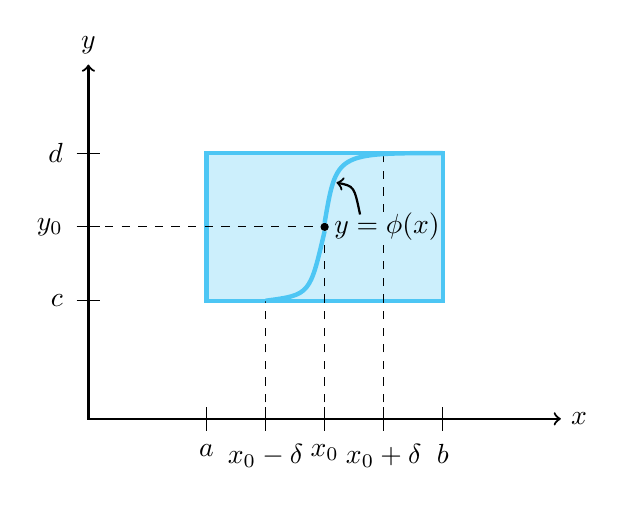
\begin{tikzpicture}[scale=1.5]
		% Draw axes
		\draw [<->,thick] (0,3) node (yaxis) [above] {$y$}
		|- (4,0) node (xaxis) [right] {$x$};
		% Draw Rectangle
		\filldraw[ultra thick][draw=cyan!70!,fill=cyan!20!] (1,1) rectangle (3,2.25);
		% Draw stuff on axes / Nodes
		\draw (1,-.1) -- (1,.1) node [below=3.5mm] {$a$};
		\draw (3,-.1) -- (3,.1) node [below=3.5mm] {$b$};
		\draw (-.1,1) -- (.1,1) node [left=3.5mm] {$c$};
		\draw (-.1,2.25) -- (.1,2.25) node [left=3.5mm] {$d$};
		\draw (2,-.1) -- (2,.1) node [below=3.5mm] {$x_0$};
		\draw (-.1,1.625) -- (.1,1.625) node [left=3.5mm] {$y_0$};
		\draw (1.5,-.1) -- (1.5,.1) node [below=3.5mm] { $x_0-\delta$};
		\draw (2.5,-.1) -- (2.5,.1) node [below=3.5mm] { $x_0+\delta$};
		\draw [fill=black] (2,1.625) circle (0.03cm) node [right] { $y=\phi(x)$};
		% Draw dashed lines
		\draw [dashed] (2,0) -- (2,1.625);
		\draw [dashed] (0,1.625) -- (2,1.625);
		\draw [dashed] (1.5,0) -- (1.5,1);
		\draw [dashed] (2.5,0) -- (2.5,1.53);
		\draw [dashed] (2.5,1.75) -- (2.5,2.25);
		% Draw curvy line
		\draw[ultra thick,cyan!70!] (1.5,1) .. controls (1.875,1.05) .. (2,1.59);
		\draw[ultra thick,cyan!70!] (2,1.66) .. controls (2.1,2.25) .. (3,2.25);
		\draw[thick,->] (2.3,1.73) .. controls (2.25,1.97) .. (2.1,2);
		\end{tikzpicture}
		\captionof{figure}{Layout for the existence-uniqueness theorem}
		\end{center}

	\noindent This theorem tells us two things. First, when an equation satisfies the hypothesis of Theorem 1.4.1, we are assured that a solution to the initial value problem exists. Naturally, it is desirable to know whether the equation we are trying to solve actually has a solution before we spend too much time trying to solve it. Second, when the hypotheses are satisfied, there is a \textit{unique} solution to the initial value problem. This uniqueness tells us that if we can find a solution, then it is the only \textit{only} solution for the initial value problem. Graphically, the theorem says that there is only one solution curve that passes through the point $ (x_0,y_0) $. In other words, for this first-order equation, two solutions cannot cross anywhere in the rectangle. Notice that the existence and uniqueness of the solution holds only in \textit{some} neighborhood $ (x_0 - \delta, x_0 + \delta) $.

	\noindent When initial value problems are used to model physical phenomena, many practitioners tactically presume the conclusions of Theorem 1.4.1 to be valid. Indeed, for the initial value problem to be a reasonable model, we certainly expect it to have a solution, since physically, ``something does not happen!''. Moreover, the solution should be unique in those cases when repetition of the experiment under identical conditions yields the same results.


	\section{Direction Fields}

	The existence-uniqueness theorem certainly has great value, but it doesn't really tell us about the \textit{nature} of the solution to a differential equation. What if we need to know the value of the solution at a certain point, or the intervals where the solution is increasing or decreasing? This is where direction fields come in.	A plot of short line segments drawn at various points in the $ xy- $plane showing the slope of the solution curve there is called a \textbf{direction field} for a differential equation. Here's a quick example:

	\begin{center}
	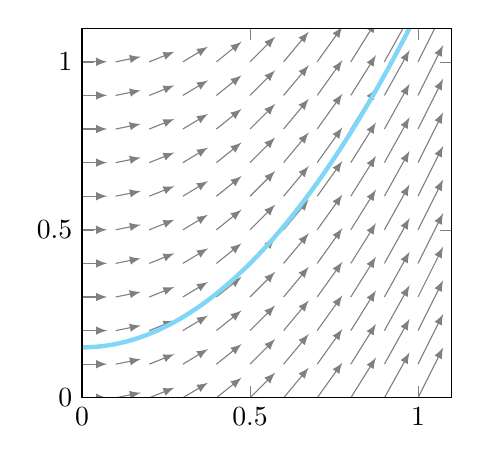
\begin{tikzpicture}[
	declare function={f(\x) = 2*\x;} % Define which function we're using
	]
	\begin{axis}[
	MaoYiyi,
	]
	\addplot3 (x,y,0);
	\addplot {x^2+0.15}; % You need to find the antiderivative yourself, unfortunately. Good exercise!
	\end{axis}
	\end{tikzpicture}
	\captionof{figure}{Direction field for $ dy/dx = 2x $ with the solution curve in blue.}
	\end{center}

	\noindent Clearly, sketches of solution fields for first-order differential equations can be helpful in visualizing the solution(s). However, such a sketch is not sufficient to enable us to trace, unambiguously, the solution curve passing through a given initial point $ (x_0,y_0) $.

	\section{Exact Differential Equations}

	Suppose we have the following differential equation
	\begin{equation}
		M(x,y) + N(x,y)\, \frac{dy}{dx} = 0
	\end{equation}
	Note that it's super important to have it in this form! Now, if there's a function somewhere in the world, $ \Psi(x,y) $, such that,
	\begin{equation}
		\frac{\partial \Psi}{\partial x} = M(x,y) \qquad \text{ and } \qquad \frac{\partial \Psi}{\partial y} = N(x,y)
	\end{equation}
	then we can call the differential equation \textit{exact}. In these cases we can write the differential equation as
	\begin{equation}
		\frac{\partial \Psi}{\partial x} + \frac{\partial \Psi}{\partial y} \frac{dy}{dx} = 0
	\end{equation}
	Then using the chain rule from Calculus III we can further reduce the differential equation to the following derivative
	\[ \frac{d}{dx}(\Psi(x,y(x))) = 0 \]
	Such that the implicit solution to the differential equation is
	\begin{equation}
		\Psi(x,y) = C
	\end{equation}
	Finding $ \Psi(x,y) $ is clearly the central task in determining if a differential equation is exact and finding its solution. But before we start, we need to see if its even exact or not before determining what $ \Psi(x,y) $ is. If a differential equation is exact, then
	\begin{equation}
		\frac{\partial M}{\partial y} = \frac{\partial N}{\partial x}
	\end{equation}
	If this is true for the differential equation that we are trying to solve, then we can proceed to find $ \Psi(x,y) $.

	\noindent \textbf{Example} Find the solution to the following initial value problem
	\[ 2xy^2+4 = 2(3-x^2y)y' \qquad y(-1) = 8 \]
	\textbf{Solution}\\
	First we need to put the differential equation into the proper form before actually solving
	\begin{align*}
		&2xy^2 + 4 - 2(3 - x^2y)y' = 0\\
		&2xy^2 + 4 + 2(x^2y - 3)y' = 0
	\end{align*}
	So now we have the following
	\begin{align*}
  		M &= 2xy^2 + 4 & \frac{\partial M}{\partial y} &= 4xy\\
  		N &= 2x^2y - 6 & \frac{\partial N}{\partial x} &= 4xy
	\end{align*}
	So the differential equation is exact. Great! We can either integrate $M$ with respect to $x$ or $N$ with respect to $y$. In this case we'll just integrate $N$.
	$$ \Psi(x,y) = \int 2x^2y - 6\,dy = x^2y^2 - 6y + h(x) $$
	Our constant of integration is going to be a function of $x$ since we integrated with respect to $y$. Now we differentiate $\Psi(x,y)$ with respect to $x$ and compare to $M$.
	$$ \frac{\partial \Psi}{\partial x} = 2xy^2 + h'(x) = 2xy^2 + 4 $$
	So it looks like
	$$ h'(x) = 4 \quad \to \quad h(x) = 4x $$
	Adding that into $\Psi(x,y)$,
	$$ \Psi(x,y) = x^2y^2 -6y + 4x $$
	So our implicit solution to the differential equation is
	$$ x^2y^2 -6y + 4x = C $$
	Applying the initial condition gives,
	$$ 64 - 48 - 4 = C $$
	$$ C = 12 $$
	The solution is then
	$$ x^2y^2 - 6y + 4x - 12 = 0 $$
	Applying the quadratic formula gives us
	\begin{align*}
		y(x) &= \frac{6 \pm \sqrt{36 - 4x^2(4x-12)}}{2x^2}\\
		&= \frac{6 \pm \sqrt{36 + 48x^2 - 16x^3}}{2x^2}\\
		&= \frac{6 \pm 1\sqrt{9 + 12x^2 - 4x^3}}{2x^2}\\
		&= \frac{3 \pm \sqrt{9 + 12x^2 - 4x^3}}{x^2}
	\end{align*}
	Reapplying the initial condition shows us that the only answer is the positive one, so our explicit solution to the differential equation is
	$$  y(x) = \frac{3 + \sqrt{9 + 12x^2 - 4x^3}}{x^2}$$

	\newpage


	\section{Euler's Method}

	Up to this point, practically every differential equation we've seen could be solved. The problem with this is most differential equation cannot be solved exactly. So what do we do when faced with a differential equation that we can’t solve?  The answer depends on what you are looking for.  If you are only looking for long term behavior of a solution you can always sketch a direction field.  This can be done without too much difficulty for some fairly complex differential equations that we can’t solve to get exact solutions.\\ \\
	The problem with this approach is that it’s only really good for getting general trends in solutions and for long term behavior of solutions.  There are times when we will need something more.  For instance, maybe we need to determine how a specific solution behaves, including some values that the solution will take.  There are also a fairly large set of differential equations that are not easy to sketch good direction fields for.\\ \\
	In these cases we resort to numerical methods that will allow us to approximate solutions to differential equations.  There are many different methods that can be used to approximate solutions to a differential equation and in fact whole classes can be taught just dealing with the various methods.  We are going to look at one of the oldest and easiest to use here.  This method was originally devised by Euler and is called, oddly enough, \textit{Euler's Method}.\\ \\
	Let's start with a general first order initial value problem
	\[ \frac{dy}{dt} = f(t,y) \qquad y(t_0) = y_0 \]
	where $ f(t,y) $ is a known function and the values in the initial condition are known numbers. Let's also assume $ f(t,y) $ is continuous so that way we'll have a solution that exists.\\ \\
	We want to approximate the solution near $ t = t_0 $. We'll start with our equation of the tangent line from Calculus I
	\[ y = y_0 + f(t_0,y_0)(t-t_0) \]
	which is shown in the figure below.

	\begin{center}
		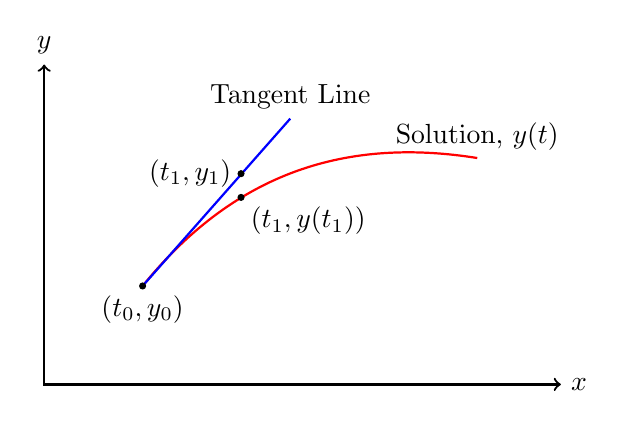
\begin{tikzpicture}[scale=1.25]
			% Draw axes
			\draw [<->,thick] (0,3.25) node (yaxis) [above] {$y$}
			|- (5.25,0) node (xaxis) [right] {$x$};
			% Curve / Tangent Line
			\draw [thick, red] (1,1) to [bend left] (4.4,2.3);
			\draw [thick, blue] (1,1) -- (2.5,2.7);
			% Nodes
			\draw (4.4,2.2) node [above=1mm] {Solution, $y(t)$};
			\draw [fill=black] (1,1) circle (0.03cm) node [below] { $(t_0,y_0)$};
			\draw (2.5,2.7) node [above] {Tangent Line};
			\draw [fill=black] (2,2.141) circle (0.03cm) node [left] { $(t_1,y_1)$};
			\draw [fill=black] (2,1.9) circle (0.03cm) node [below right] { $(t_1,y(t_1))$};
		\end{tikzpicture}
		\captionof{figure}{Tangent Line of Solution Curve}
	\end{center}

	\noindent If $ t_1 $ is close enough to $ t_0 $ then the point $ y_1 $ on the tangent line should be fairly close to the actual value of the solution at $ t_1 $, or $ y(t_1) $. Finding $ y_1 $ is easy enough. All we need to do is plug $ t_1 $ in the equation for the tangent line
	\[ y_1 = y_0 + f(t_0,y_0)(t_1-t_0) \]
	Now, we would like to proceed in a similar manner, but we don't have the solution at $ t_1 $ and so we won't know the slope of the tangent line to the solution at this point, which is a problem! We can partially solve it, however, by recalling that $ y_1 $ is an approximation to the solution at $ t_1 $. If $ y_1 $ is a very good approximation to the actual value of the solution then we can use that to estimate the slope of the tangent line at $ t_1 $.

	\noindent So, let's hope that $ y_1 $ is a good approximation to the solution and construct a line through the point $ (t_1,y_1) $ that has a slope $ f(t_1,y_1) $. This gives
	\[ y = y_1 + f(t_1,y_1)(t-t_1) \]
	Now, to get an approximation to the solution at $ t = t_2 $ we will hope that this new line will be fairly close to the actual solution at $ t_2 $ and use the value of the line at $ t_2 $ as an approximation to the actual solution. This gives
	\[ y = y_1 + f(t_1,y_1)(t_2-t_1) \]
	We can continue in this fashion. Use the previously computed approximation to get the next approximation. So,
	\begin{align*}
		y_3 &= y_2+f(t_2,y_2)(t_3-t_2)\\
		y_4 &= y_3+f(t_3,y_3)(t_4-t_2)\\
		& \qquad \qquad \vdots\\
		y_{n+1} &= y_n + f(t_n,y_n)(t_{n+1}-t_n)
	\end{align*}
	If we define $ f_n = f(t_n,y_n) $ we can further simplify the formula to
	\[ y_{n+1} = y_n + f_n \cdot (t_{n+1} - t_n) \]
	We will often assume that the step sizes between the points $ t_0,t_1,t_2, \dots, t_n $ are of uniform size of $ h $. In other words,
	\[ t_{n+1} - t_n = h \]
	This doesn’t have to be done and there are times when it’s best that we not do this.  However if we do, the formula for the next approximation becomes.
	\begin{equation}
		y_{n+1} = y_n + hf_n
	\end{equation}


	\begin{center}
		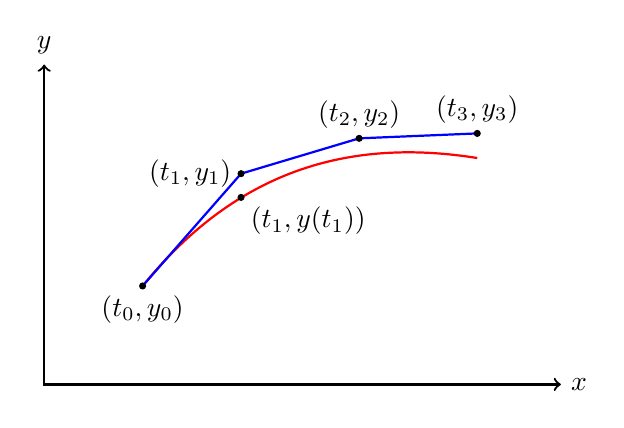
\begin{tikzpicture}[scale=1.25]
		% Draw axes
		\draw [<->,thick] (0,3.25) node (yaxis) [above] {$y$}
		|- (5.25,0) node (xaxis) [right] {$x$};
		% Curve / Tangent Line
		\draw [thick, red] (1,1) to [bend left] (4.4,2.3);
		\draw [thick, blue] (1,1) -- (2,2.141);
		\draw [thick, blue] (2,2.141) -- (3.2,2.5);
		\draw [thick, blue] (3.2,2.5) -- (4.4,2.55);
		% Nodes
		\draw [fill=black] (1,1) circle (0.03cm) node [below] { $(t_0,y_0)$};
		\draw [fill=black] (3.2,2.5) circle (0.03cm) node [above] { $(t_2,y_2)$};
		\draw [fill=black] (4.4,2.55) circle (0.03cm) node [above] { $(t_3,y_3)$};
		\draw [fill=black] (2,2.141) circle (0.03cm) node [left] { $(t_1,y_1)$};
		\draw [fill=black] (2,1.9) circle (0.03cm) node [below right] { $(t_1,y(t_1))$};
		\end{tikzpicture}
		\captionof{figure}{Illustration of Euler's Method}
	\end{center}

	\noindent In practice you would need to write a computer program to do these computations for you.  In most cases the function $ f(t,y) $ would be too large and/or complicated to use by hand and in most serious uses of Euler’s Method you would want to use hundreds of steps which would make doing this by hand prohibitive.  So, here is a bit of pseudo-code that you can use to write a program for Euler’s Method that uses a uniform step size, $ h $.

	\begin{lstlisting}[frame=none,numbers=none]
	define f(t,y)
	input t0 and y0
	input h and number of steps n
	for j from 1 to n do
		m = f(t0,y0)
		y1 = y0 + h*m
		t1 = t0 + h
		Print t1 and y1
		t0 = t1
		y0 = y1
	end
	\end{lstlisting}

	\noindent \textbf{Example} Use Euler's method with step size $ h = 0.25 $ to find $ f(1) $ for the initial value problem
	\[ y' = 2 - e^{-4t} -2y \qquad y(0) = 1 \]
	\textbf{Solution}\\
	We see that $ f(t,y) = 2 - e^{-4t} - 2y $ and $ t_0 = 0, y_0 = 1 $. Now we can start doing some calculations.

	\noindent Step 1
	\begin{align*}
		& f(0,1) = 2 - e^{-4(0)} - 2(1) = -1\\
		& y_1 = 1 + (0.25)(-1) = 0.75
	\end{align*}

	\noindent Step 2
	\begin{align*}
		& f(0.25,0.75) = 2 - e^{-4(0.25)} - 2(0.75) = 0.132121\\
		& y_2 = 0.75 + (0.25)(0.132121) = 0.78303
	\end{align*}

	\noindent We'll continue and put all of our values into this nifty table
	\begin{center}
	\begin{tabular}{c|c|c}
		$t$  &   $y$    & $f(t,y)$ \\ \hline
		0	 &    1     &    -1    \\
		0.25 &   0.75   & 0.132121 \\
		0.5  & 0.78303  & 0.298604 \\
		0.75 & 0.857681 & 0.23485  \\
		1    & 0.916394 & 0.148897
	\end{tabular}
	\end{center}
	So $ y(1) \approx 0.916394 $.

	\chapter{Second Order Differential Equations}\normalsize
	In the previous chapter we looked at first order differential equations. In this chapter we will move on to second order differential equations. Just as we did in the last chapter we will look at some special cases of second order differential equations that we can solve. Unlike the previous chapter however, we are going to have to be even more restrictive as to the kinds of differential equations that we’ll look at. This will be required in order for us to actually be able to solve them.

	\section{Introduction}

	In this chapter we will be looking exclusively at linear second order differential equations.  The most general linear second order differential equation is in the form
	\begin{equation}
		p(t)y'' + q(t)y' + r(t)y = g(t)
	\end{equation}
	In fact, we will rarely look at non-constant coefficient linear second order differential equations.  In the case where we assume constant coefficients we will use the following differential equation
	\begin{equation}
		ay'' + by' + cy = g(t)
	\end{equation}
	When $ g(t) = 0 $ we call the differential equation \textit{homogeneous} and when $ g(t) \neq 0 $ we call the differential equation \textit{nonhomogeneous}.

	\noindent \textbf{Principle of Superposition}

	\noindent If $ y_1(t) $ and $ y_2(t) $ are solutions to a linear, homogeneous differential equation then so is
	\[ y(t) = c_1y_1(t) + c_2y_2(t) \]
	Note that we didn’t include the restriction of constant coefficient or second order in this.  This will work for any linear homogeneous differential equation.

	\noindent \textbf{Example} Solve the following initial value problem
	\[ y'' - 9y = 0 \qquad y(0) = 2 \qquad y'(0) = -1 \]
	\textbf{Solution}\\
	We see that there are two answers to this differential equation
	\[ y(t) = e^{-3t} \qquad \text{and} \qquad y(t) = e^{3t} \]
	The general solution to our differential equation is then
	\[ y(t) = c_1e^{-3t} + c_2e^{3t} \]
	It may not make a whole lot of sense right now but it will in later sections.

	\noindent Now all we need to do is apply the initial conditions.  This means that we need the derivative of the solution.
	\[ y'(t) = -3c_1e^{3t} + 3c_2e^{3t} \]
	Plug in the initial conditions
	\begin{align*}
		2 &= c_1 + c_2\\
		-1 &= -3c_1 + 3c_2
	\end{align*}
	Giving us a system of equations to solve. After doing a little algebra we find that
	\[ c_1 = \frac{7}{6} \qquad c_2 = \frac{5}{6} \]
	Therefore the solution to the initial value problem is
	\[ y(t) = \frac{7}{6}e^{-3t} + \frac{5}{6}e^{3t} \]

	\section{The Characteristic Equation}

	Let's assume that the differential equation
	\begin{equation}
		ay'' + by' + cy = 0
	\end{equation}
	has the form
	\begin{equation}
		y = e^{rt}
	\end{equation}
	To see if we're right we'll just plug it back in to the differential equation. So take 2 derivatives and plug everything in.
	\[ y = e^{rt} \qquad y' = re^{rt} \qquad y'' = r^2 e^{rt} \]
	\begin{align*}
		a(r^2 e^{rt}) + b(re^{rt}) + c(e^{rt}) &= 0\\
		e^{rt}(ar^2 + br + c) &= 0
	\end{align*}
	Since exponentials are never zero then that means that
	\begin{equation}
		ar^2 + br + c = 0
	\end{equation}
	This equation is typically called the \textit{characteristic equation}. Since the characteristic equation is in the form of a quadratic then the two solutions are
	\[ r = \frac{-b \pm \sqrt{b^2 - 4ac}}{2a} \]
	So there will be three cases for $ r $.
	\begin{enumerate}
		\item Real, distinct roots: $ r_1 \neq r_2 $
		\item Complex roots: $ r_{1,2} = \alpha \pm \beta i $
		\item Repeating roots: $ r_1 = r_2 $
	\end{enumerate}
	The next three sections will look at each of these in some more depth, including giving forms for the solution that will be “nice enough” to get a general solution.

	\section{Real, Distinct Roots}

	Recall that to solve the differential equation
	\[ ay'' + by' + cy = 0 \]
	We set up the characteristic equation
	\[ ar^2 + br + c = 0 \]
	Since this is a quadratic, we will have two solutions $ r_1 $ and $ r_2 $. So the solution to the differential equation are
	\[ y(t) = c_1e^{r_1 t} + c_2e^{r_2 t} \]

	\noindent \textbf{Example} Solve the following differential equation
	\[ y'' - 6y' - 2y = 0 \]
	\textbf{Solution}\\
	The characteristic equation is
	\[ r^2 - 6r - 2 \]
	and the roots are
	\[ r = 3 \pm \sqrt{11} \]
	So the solution to the differential equations is
	\[ y(t) = c_1e^{(3 + \sqrt{11})t} + c_2e^{(3 - \sqrt{11})t} \]

	\section{Complex Roots}

	If our differential equation is in the form
	\[ ay'' + by' + cy = 0 \]
	then we set up the characteristic equation
	\[ ar^2 + br + c = 0 \]
	If this has complex roots of the form $ r_{1,2} = \alpha \pm i \beta $, then the solution would be
	\[ y(t) = c_1 e^{(\alpha + i \beta)t} + c_2 e^{(\alpha - i \beta)t} \]
	We do have a problem however.  Since we started with only real numbers in our differential equation we would like our solution to only involve real numbers.  The two solutions above are complex and so we would like to get our hands on a couple of solutions that are real. To do this we need Euler's formula
	\[ e^{i\theta} = \cos(\theta) + i\sin(\theta) \]
	and a nice variant of it
	\[ e^{-i\theta} = \cos(-\theta) + i\sin(-\theta) = \cos(\theta) - i\sin(\theta) \]
	Now, split up our two solutions into exponentials that only have real exponents and exponentials that only have imaginary exponents. Then use Euler’s formula, and its variant, to rewrite the second exponential.
	\begin{align*}
		y_1(t) &= e^{\alpha t} e^{i \beta t} = e^{\alpha t}(\cos(\beta t) + i\sin(\beta t))\\
		y_2(t) &= e^{\alpha t} e^{-i \beta t} = e^{\alpha t}(\cos(\beta t) - i\sin(\beta t))
	\end{align*}
	This doesn’t eliminate the complex nature of the solutions, but it does put the two solutions into a form that we can eliminate the complex parts.\\ \\
	Notice that if we add the two solutions together we will arrive at
	\[ y_1(t) + y_2(t) = 2e^{\alpha t} \cos(\beta t) \]
	This is a real solution and just to eliminate the extraneous 2 let’s divide everything by a 2. This gives the first real solution that we’re after
	\[ u(t) = \frac{1}{2}y_1(t) + \frac{1}{2}y_2(t) = e^{\alpha t} \cos(\beta t) \]
	Note that this is just equivalent to taking
	\[ c_1 = c_2 = \frac{1}{2} \]
	Now, we can arrive at a second solution in a similar manner.  This time let’s subtract the two original solutions to arrive at
	\[ y_1(t) - y_2(t) = 2i e^{\alpha t} \sin(\beta t) \]
	On the surface this doesn't appear to fix the problem as the solution is still complex.  However, upon learning that the two constants, $ c_1 $ and $ c_2 $ can be complex numbers we can arrive at a real solution by dividing this by $ 2i $.  This is equivalent to taking
	\[ c_1 = \frac{1}{2i} \qquad \text{and} \qquad c_2 = -\frac{1}{2i} \]
	Our second solution will then be
	\[ v(t) = \frac{1}{2i} y_1(t) - \frac{1}{2i} y_2(t) = e^{\alpha t} \sin(\beta t) \]
	We now have two solutions to the differential equation
	\[ u(t) = e^{\alpha t} \cos(\beta t) \qquad \text{and} \qquad v(t) = e^{\alpha t} \sin(\beta t)  \]
	So, if the roots of the characteristic equation happen to be $ r_{1,2} = \alpha \pm i \beta $, the general solution to the differential equation is
	\begin{align*}
		y(t) &= c_1 e^{\alpha t}\cos(\beta t) + c_2 e^{\alpha t}\sin(\beta t)\\
		&= e^{\alpha t}(c_1\cos(\beta t) + c_2\sin(\beta t))
	\end{align*}

	\section{Repeated Roots}

	In this section we will be looking at the last case for the constant coefficient, linear, homogeneous second order differential equations.  In this case we want solutions to
	\[ ay'' + by' + cy = 0 \]
	where solutions to the characteristic equation
	\[ ar^2 + br + c = 0 \]
	are double roots $ r_1 = r_2 = r $.\\ \\
	This leads to a problem however.  Recall that the solutions are
	\[ y_1(t) = e^{r_1 t} = e^{rt} \qquad y_2(t) = e^{r_2 t} = e^{rt} \]
	These are the same solution and will \textbf{not} be nice enough to form a general solution. So, we can use the first solution, but we're going to need a second solution.\\ \\
	From the quadratic formula we know that the roots to the characteristic equation are,
	\[ r_{1,2} = \frac{-b \pm \sqrt{b^2 - 4ac}}{2a} \]
	In this case, since we have double roots we must have
	\[ b^2 - 4ac = 0 \]
	This is the only way that we can get double roots and in this case the roots will be
	\[ r_{1,2} = \frac{-b}{2a} \]
	So, the one solution that we've got is
	\[ y_1(t) = e^{\left(\frac{-b}{2a}\right)t} \]
	To find a second solution we will use the fact that a constant times a solution to a linear homogeneous differential equation is also a solution. If this is true then \textit{maybe} we'll get lucky and the following will also be a solution
	\begin{equation}
		y_2(t) = v(t)y_1(t) = v(t)e^{\left(\frac{-b}{2a}\right)t}
	\end{equation}
	with a proper choice of $ v(t) $.  To determine if this in fact can be done, let’s plug this back into the differential equation and see what we get.  We'll first need a couple of derivatives.
	\begin{align*}
		y_2'(t) &= v' e^{\left(\frac{-b}{2a}\right)t} - \frac{b}{2a} v e^{\left(\frac{-b}{2a}\right)t} \\
		y_2''(t) &= v'' e^{\left(\frac{-b}{2a}\right)t} - \frac{b}{2a} v' e^{\left(\frac{-b}{2a}\right)t} - \frac{b}{2a} v' e^{\left(\frac{-b}{2a}\right)t} + \frac{b^2}{4a^2} v e^{\left(\frac{-b}{2a}\right)t}\\
		&= v'' e^{\left(\frac{-b}{2a}\right)t} - \frac{b}{a} v' e^{\left(\frac{-b}{2a}\right)t} + \frac{b^2}{4a^2} v e^{\left(\frac{-b}{2a}\right)t}
	\end{align*}
	Now, plug these into the differential equation.
	\[ a\left( v'' e^{\left(\frac{-b}{2a}\right)t} - \frac{b}{a} v' e^{\left(\frac{-b}{2a}\right)t} + \frac{b^2}{4a^2} v e^{\left(\frac{-b}{2a}\right)t} \right) + b\left( v' e^{\left(\frac{-b}{2a}\right)t} - \frac{b}{2a} v e^{\left(\frac{-b}{2a}\right)t} \right) + c \left( v e^{\left(\frac{-b}{2a}\right)t} \right) = 0 \]
	We can factor an exponential out of all the terms so let's do that.  We'll also collect all the coefficients of $ v $ and its derivatives.
	\begin{align*}
		e^{\left(\frac{-b}{2a}\right)t} \left( av'' + (-b + b)v' + \left( \frac{b^2}{4a} - \frac{b^2}{2a} + c \right)v \right) &= 0\\
		e^{\left(\frac{-b}{2a}\right)t} \left( av'' + \left( -\frac{b^2}{4a} + c \right) v \right) &= 0\\
		e^{\left(\frac{-b}{2a}\right)t} \left( av'' - \frac{1}{4a}(b^2 - 4ac) v \right) &= 0
	\end{align*}
	Now, because we are working with a double root we know that that the second term will be zero.  Also exponentials are never zero.  Therefore, Equation 2.6 will be a solution to the differential equation provided $ v(t) $ is a function that satisfies the following differential equation
	\[ av'' = 0 \qquad \text{or} \qquad v'' = 0 \]
	We can drop the $ a $ because we know that it can't be zero. If it were we wouldn't have a second order differential equation!  So, we can now determine the most general possible form that is allowable for $ v(t) $
	\[ v' = \int v''\,dt = c \qquad v(t) = \int v'\,dt = ct + k \]
	This is actually more complicated than we need and in fact we can drop both of the constants from this. To see why this is let's go ahead and use this to get the second solution. The two solutions are then
	\[ y_1(t) = e^{\left(\frac{-b}{2a}\right)t} \qquad y_2(t) = (ct + k) e^{\left(\frac{-b}{2a}\right)t} \]
	The general solution would then be the following
	\begin{align*}
		y(t) &= c_1 e^{\left(\frac{-b}{2a}\right)t} + c_2 (ct + k) e^{\left(\frac{-b}{2a}\right)t}\\
		&= c_1 e^{\left(\frac{-b}{2a}\right)t} + (c_2 ct + c_2 k) e^{\left(\frac{-b}{2a}\right)t}\\
		&= (c_1 + c_2 k)e^{\left(\frac{-b}{2a}\right)t} + c_2 c e^{\left(\frac{-b}{2a}\right)t}
	\end{align*}
	Now, $ c,\, k,\, c_1 $, and $ c_2 $ are all unknown constants so any combination of them will also be unknown constants.  In particular, $c_1+c_2, \, k$ and  $c_2, \, c$ are unknown constants so we'll just rewrite them as follows
	\[ y(t) = c_1 e^{\left(\frac{-b}{2a}\right)t} + c_2 t e^{\left(\frac{-b}{2a}\right)t} \]
	Let's recap.  If the roots of the characteristic equation are $ r_1 = r_2 = r $, then the general solution is then
	\[ y(t) = c_1 e^{rt} + c_2 t e^{rt} \]

	\section{Undetermined Coefficients}

	In this section we will take a look at the first method that can be used to find a particular solution to a nonhomogeneous differential equation
	\[ y'' + p(t)y' + q(t)y = g(t) \]
	One of the main advantages of this method is that it reduces the problem down to an algebra problem. The algebra can get messy on occasion, but for most of the problems it will not be terribly difficult. Another nice thing about this method is that the complementary solution will not be explicitly required, although as we will see knowledge of the complementary solution will be needed in some cases and so we'll generally find that as well.\\ \\
	There are two disadvantages to this method.  First, it will only work for a fairly small class of $ g(t) $'s.  The class of $ g(t) $'s for which the method works, does include some of the more common functions, however, there are many functions out there for which undetermined coefficients simply won't work. Second, it is generally only useful for constant coefficient differential equations.\\ \\
	The method is quite simple. All that we need to do is look at $ g(t) $ and make a guess as to the form of $ y_p(t) $ leaving the coefficient(s) undetermined (hence the name of the method). Plug the guess into the differential equation and see if we can determine values of the coefficients. If we can determine values for the coefficients then we guessed correctly, if we can’t find values for the coefficients then we guessed incorrectly.It's usually easier to see this method in action rather than to try and describe it, so let's jump into some examples.

	\noindent \textbf{Example} Determine the solution to
	\[ y'' - 4y' - 12y = 3e^{5t} \]
	\textbf{Solution}\\
	The point here is to find a particular solution, however the first thing that we’re going to do is find the homogeneous solution to this differential equation. Recall that the homogeneous solution comes from solving,
	\[ y'' - 4y' - 12y = 0 \]
	The characteristic equation for this differential equation and its roots are
	\[ r^2 - 4r - 12 = (r - 6)(r + 2) = 0 \qquad \Rightarrow \qquad r_1 = -2, r_2 = 6 \]
	The homogeneous solution is then,
	\[ y_h(t) = c_1 e^{-2t} + c_2 e^{6t} \]
	Now, let's proceed with finding a particular solution. As mentioned prior to the start of this example we need to make a guess as to the form of a particular solution to this differential equation. Since $ g(t) $ is an exponential and we know that exponentials never just appear or disappear in the differentiation process it seems that a likely form of the particular solution would be
	\[ y_p(t) = Ae^{5t} \]
	Now, all that we need to do is do a couple of derivatives, plug this into the differential equation and see if we can determine what $ A $ needs to be. Plugging into the differential equation gives
	\begin{align*}
		25Ae^{5t} - 4(5Ae^{4t}) - 12(Ae^{5t}) &= 3e^{5t}\\
		-7Ae^{5t} &= 3e^{5t}\\
		A &= -\frac{3}{7}
	\end{align*}
	Okay, we found a value for the coefficient. This means that we guessed correctly. A particular solution to the differential equation is then,
	\[ y_p(t) = -\frac{3}{7}e^{5t} \]
	Since the solution is in the form $ y(t) = y_h(t) + y_p(t) $, the solution is then
	\[ y(t) = c_1 e^{-2t} + c_2 e^{6t} -\frac{3}{7}e^{5t} \]
	Let's take a look at another example that will give the second type of $ g(t) $ for which undetermined coefficients will work.

	\noindent \textbf{Example} Find a particular solution for the following differential equation.
	\[ y'' - 4y' - 12y = \sin(2t) \]
	\textbf{Solution}\\
	Now, let's take our experience from the first example and apply that here.  The first example had an exponential function in the $ g(t) $ and our guess was an exponential. This differential equation has a sine so let’s try the following guess for the particular solution.
	\[ y_p(t) = A\sin(2t) \]
	Differentiating and plugging into the differential equation gives,
	\[ -4A\sin(2t) - 4(2A\cos(2t)) - 12(A\sin(2t)) = \sin(2t) \]
	Collecting like terms yields
	\[ -16A\sin(2t) - 8A\cos(2t) = \sin(2t) \]
	We need to pick $ A $ so that we get the same function on both sides of the equal sign. This means that the coefficients of the sines and cosines must be equal. Or,
	\begin{center}
	\begin{tabular}{lcll}
		$\cos(2t):$ & $-8A = 0$ & $\Rightarrow$ & $A = 0$\\
		$\sin(2t):$ & $-16A = 1$ & $\Rightarrow$ & $\displaystyle{A = -\frac{1}{16}}$
	\end{tabular}
	\end{center}
	Notice two things. First, since there is no cosine on the right hand side this means that the coefficient must be zero on that side. More importantly we have a serious problem here. In order for the cosine to drop out, as it must in order for the guess to satisfy the differential equation, we need to set $ A = 0 $, but if $ A = 0 $, the sine will also drop out and that can't happen. Likewise, choosing $ A $ to keep the sine around will also keep the cosine around. What this means is that our initial guess was wrong. If we get multiple values of the same constant or are unable to find the value of a constant then we have guessed wrong. \\ \\
	One of the nicer aspects of this method is that when we guess wrong our work will often suggest a fix.  In this case the problem was the cosine that cropped up.  So, to counter this let’s add a cosine to our guess.  Our new guess is
	\[ y_p(t) = A\cos(2t) + B\sin(2t) \]
	Plugging this into the differential equation and collecting like terms gives,
	\begin{align*}
		-4A\cos(2t) - 4B\sin(2t) - 4(-2A\sin(2t) + 2B\cos(2t)) - 12(A\cos(2t) + B\sin(2t)) &= \sin(2t)\\
		(-4A - 8B - 12A)\cos(2t) + (-4B + 8A -12B)\sin(2t) &= \sin(2t)\\
		(-16A - 8B)\cos(2t) + (8A - 16B)\sin(2t) &= \sin(2t)
	\end{align*}
	Now, set the coefficients equal
	\begin{align*}
	\cos(2t): \quad -16A - 8B &= 0\\
	\sin(2t): \qquad 8A - 16B &= 1
	\end{align*}
	Solving this system gives us
	\[ A = \frac{1}{40} \qquad B = -\frac{1}{20} \]
	We found constants and this time we guessed correctly. A particular solution to the differential equation is then,
	\[ y_p(t) = \frac{1}{40}\cos(2t) - \frac{1}{20}\sin(2t) \]
	Notice that if we had had a cosine instead of a sine in the last example then our guess would have been the same. In fact, if both a sine and a cosine had shown up we will see that the same guess will also work.\\ \\
	Let's take a look at the third and final type of basic $ g(t) $ that we can have. There are other types of $ g(t) $ that we can have, but as we will see they will all come back to two types that we've already done as well as the next one.\\ \\
	\textbf{Example} Find a particular solution for the following differential equation
	\[ y'' - 4y' - 12y = 2t^3 -t + 3 \]
	\textbf{Solution}\\
	For this example $ g(t) $ is a third degree polynomial. For this we will need the following guess for the particular solution
	\[ y_p(t) = At^3 + Bt^2 + Ct + D \]
	Notice that even though $ g(t) $ doesn't have a t2 in it our guess will still need one!  So, differentiate and plug into the differential equation.
	\begin{align*}
		6At + 2B - 4(3At^2 + 2Bt + C) - 12(At^3 + Bt^2 + Ct + D) &= 2t^3 - t + 3\\
		-12At^3 + (-12A - 12B)t^2 + (6A - 8B - 12C)t + 2B - 4C - 12D &= 2t^3 - t + 3
	\end{align*}
	Now, as we've done in the previous examples we will need the coefficients of the terms on both sides of the equal sign to be the same so set coefficients equal and solve.
	\begin{center}
	\begin{tabular}{lcll}
		$ t^3: $ & $ -12A =2 $  & $ \Rightarrow $ & $ \displaystyle{A = -\frac{1}{6}} $ \\
		$ t^2: $ & $ -12A - 12B = 0 $ & $ \Rightarrow $ & $ \displaystyle{B = \frac{1}{6}} $  \\
		$ t^1: $   & $ 6A - 8B - 12C = -1 $ & $ \Rightarrow $ & $ \displaystyle{C = -\frac{1}{9}}$ \\
		$ t^0: $ & $ 2B - 4C - 12D = 3 $ & $ \Rightarrow $ & $ \displaystyle{D =\, -\frac{5}{27}} $
	\end{tabular}
	\end{center}
	A particular solution for this differential equation is then
	\[ y_p(t) = -\frac{1}{6}t^3 + \frac{1}{6}t^2 - \frac{1}{9}t - \frac{5}{27} \]
	Now that we've gone over the three basic kinds of functions that we can use undetermined coefficients on let's summarize.
	\begin{center}
		\begin{tabular}{c|c}
			$ g(t) $ & $ y_p(t) $ guess \\ \hline
			$ a e^{\beta t} $ & $ A e^{\beta t} $\\
			$ a \cos(\beta t) $ & $ A \cos(\beta t) + B\sin(\beta t) $\\
			$ b \sin(\beta t) $ & $ A \cos(\beta t) + B\sin(\beta t) $\\
			$ a \cos(\beta t) + b \sin(\beta t) $ & $ A \cos(\beta t) + B\sin(\beta t) $\\
			$ n^{th} $ degree polynomial & $ A_n t^n + A_{n-1} t^{n-1} + \dots A_1 t + A_0 $
		\end{tabular}
	\end{center}
	Notice that there are really only three kinds of functions given above.  If you think about it the single cosine and single sine functions are really special cases of the case where both the sine and cosine are present.

	\section{Variation of Parameters}
	In the last section we looked at the method of undetermined coefficients for finding a particular solution to
	\begin{equation}
		p(t)y'' + q(t)y' + r(t)y = g(t)
	\end{equation}
	and we saw that while it reduced things down to just an algebra problem, the algebra could become quite messy.  On top of that undetermined coefficients will only work for a fairly small class of functions.\\ \\
	The method of Variation of Parameters is a much more general method that can be used in many more cases. However, there are two disadvantages to the method.  First, the homogeneous solution is absolutely required to do the problem. This is in contrast to the method of undetermined coefficients where it was advisable to have the homogeneous solution on hand, but was not required. Second, as we will see, in order to complete the method we will be doing a couple of integrals and there is no guarantee that we will be able to do the integrals. So, while it will always be possible to write down a formula to get the particular solution, we may not be able to actually find it if the integrals are too difficult or if we are unable to find the homogeneous solution.\\ \\
	We're going to derive the formula for variation of parameters. We'll start off by acknowledging that the homogeneous solution to (2.7) is
	\[ y_h(t) = c_1 y_1(t) + c_2 y_2(t) \]
	What we’re going to do is see if we can find a pair of functions, $ u_1(t) $ and $ u_2(t) $ so that
	\[ y_p(t) = u_1(t) y_1(t) + u_2(t) y_2(t)  \]
	will be a solution to (2.7).  We have two unknowns here and so we'll need two equations eventually.  One equation is easy.  Our proposed solution must satisfy the differential equation, so we'll get the first equation by plugging our proposed solution into (2.7).  The second equation can come from a variety of places.  We are going to get our second equation simply by making an assumption that will make our work easier.\\ \\
	If we're going to plug our proposed solution into the differential equation we're going to need some derivatives so let's get those. The first derivative is
	\[ y_p'(t) = u_1' y_1 + u_1 y_1' + u_2' y_2 + u_2 y_2' \]
	Here's the assumption. Simply to make the first derivative easier to deal with we are going to assume that whatever $ u_1(t) $ and $ u_2(t) $ are they will satisfy the following.
	\begin{equation}
		u_1' y_1 + u_2' y_2 = 0
	\end{equation}
	Now, there is no reason ahead of time to believe that this can be done. However, we will see that this will work out. We simply make this assumption on the hope that it wo'’t cause problems down the road and to make the first derivative easier so don’t get excited about it. With this assumption the first derivative becomes
	\[ y_p'(t) = u_1 y_1' + u_2 y_2' \]
	The second derivative is then
	\[ y_p''(t) = u_1 y_1'' + u_1' y_1' + u_2 y_2'' + u_2' y_2' \]
	Plug the solution and its derivatives into (2.7).
	\[ p(t)(u_1 y_1'' + u_1' y_1' + u_2 y_2'' + u_2' y_2') + q(t)(u_1 y_1' + u_2 y_2') + r(t)(u_1 y_1 + u_2 y_2) = g(t) \]
	Rearranging a little gives the following,
	\[ p(t)(u_1' y_1' + u_2' y_2') + u_1(p(t)y_1'' + q(t)y_1' + r(t)y_1) + u_2(p(t)y_2'' + q(t)y_2' + r(t)y_2) = g(t) \]
	Now, both $ y_1 $ and $ y_2 $ are solutions to homogeneous differential equation and so the second and third terms are zero. Acknowledging this and rearranging a little gives us,
	\[ p(t)(u_1' y_1' + u_2' y_2') + u_1(0) + u_2(0) = g(t) \]
	\begin{equation}
		u_1' y_1' + u_2' y_2' = \frac{g(t)}{p(t)}
	\end{equation}
	We've almost got the two equations that we need. Before proceeding we're going to go back and make a further assumption. The last equation, (2.9), is actually the one that we want, however, in order to make things simpler for us we are going to assume that the function $ p(t) = 1 $. In other words, we are going to go back and start working with the differential equation,
	\[ y'' + q(t)y' + r(t)y = g(t) \]
	If the coefficient of the second derivative isn't one divide it out so that it becomes a one. The formula that we're going to be getting will assume this!  Upon doing this the two equations that we want so solve for the unknown functions are
	\begin{equation}
		u_1' y_1 + u_2' y_2 = 0
	\end{equation}
	\begin{equation}
		u_1' y_1' + u_2' y_2' = g(t)
	\end{equation}
	Note that in this system we know the two solutions and so the only two unknowns here are $ u_1' $ and $ u_2' $. Solving this system is actually quite simple.  First, solve (2.10) for and plug this into (2.11) and do some simplification.
	\begin{equation}
		u_1' = -\frac{u_2' y_2}{y_1}
	\end{equation}
	\begin{align*}
		\left( -\frac{u_2' y_2}{y_1} \right)y_1' + u_2 ' y_2' &= g(t)\\
		u_2' \left( y_2' - \frac{y_2 y_1'}{y_1} \right) &= g(t)\\
		u_2' \left( \frac{y_1 y_2' - y_2 y_1'}{y_1} \right) &= g(t)
	\end{align*}
	\begin{equation}
		u_2 ' = \frac{y_1 g(t)}{y_1 y_2' - y_2 y_1'}
	\end{equation}
	So, we now have an expression for $ u_2' $. Plugging this into (2.12) will give us an expression for $ u_1' $.
	\begin{equation}
		u_1' = -\frac{y_2 g(t)}{y_1 y_2' - y_2 y_1'}
	\end{equation}
	Notice the denominator is the same for (2.13) and (2.14). This is no coincidence. The name for this is the \textit{Wronskian}. It is solution to this determinant
	\[ W(y_1,y_2) =
	\begin{vmatrix}
		y_1 & y_2\\
		y_1' & y_2'
	\end{vmatrix}
	= y_1 y_2' - y_2 y_1' \]
	Finally, all that we need to do is integrate (2.13) and (2.14) in order to determine what $ u_1(t) $ and $ u_2(t) $ are. Doing this gives,
	\[ u_1(t) = -\int \frac{y_2 g(t)}{W(y_1,y_2)}\,dt \qquad u_2(t) = \int \frac{y_1 g(t)}{W(y_1,y_2)}\,dt  \]
	So, provided we can do these integrals, a particular solution to the differential equation is
	\begin{align*}
		y_p(t) &= y_1 u_1 + y_2 u_2\\
		&= -y_1 \int \frac{y_2 g(t)}{W(y_1,y_2)}\,dt + y_2 \int \frac{y_1 g(t)}{W(y_1,y_2)}\,dt
	\end{align*}
	
	\section{Euler's Method: Revisited}
	
	In the last chapter we talked about how to numerically approximate first order differential equations using Euler's Method. We can use this technique to approximate second order differential equations, but we need to do a little prep-work first.\\ \\
	Consider the following differential equation.
	\[ f''(t) + f'(t) - t(f(t))^2 \qquad f(0)=1 \quad f'(0)=1 \]
	Find $ f(1) $\\ \\
	We need to use Euler's Method on this, since this differential equation is not linear. However, we have run into a problem, Euler's Method only works for first order differential equations and this is a second order. How do we solve this? The answer is actually quite simple. We are actually going to convert this second order differential equation into a first order differential equation by introducing the following,
	\begin{align*}
		g_1(t) &= f(t)\\
		g_2(t) &= f'(t)
	\end{align*}
	Now, if we take a derivative,
	\begin{align*}
		g_1'(t) &= f'(t)\\
		g_2'(t) &= f''(t)
	\end{align*}
	Notice now we have only first order differential equations in terms of $ g(t) $'s and not $ f(t) $'s. If we finish substituting everything in terms of $ g(t) $, we have the following system,
	\begin{align*}
		g_1'(t) &= g_2(t)\\
		g_2'(t) &= t - g_2(t) + t(g_1(t))^2
	\end{align*}
	We're just forgetting one thing, we still need to convert our initial conditions into terms of $ g(t) $. Doing this yields, 
	\[ g_1(0) = 1 \qquad g_2(0)=1 \]
	Now we can perform Euler's Method! Lets use a step size of 0.25 and start doing some calculations\\ \\
	Step 1
	\[ g_2'(0) = 0 - 1 + 0(1)^2 = -1 \]
	We can now fill in our first row of our table
	
	\begin{center}
		\begin{tabular}{|c|c|c|c|c|} \hline
			$ t $ & $ g_1 $ & $ g_2 $ & $ g_1' $ & $ g_2' $ \\ \hline
			0 & 1 & 1 & 1 & -1 \\ \hline
			0.25 & & & & \\ \hline
			0.5 & & & & \\ \hline 
			0.75 & & & & \\ \hline 
			1 & & & & \\ \hline
		\end{tabular}
	\end{center}
	Step 2
	\[ g_1 = 1 + 0.25(1) = 1.25 \]
	\[ g_2 = 1 + 0.25(-1) = 0.75 \]
	\[ g_2'(0.25) = 0.25 - 0.75 + (0.75)(1.25)^2 = -0.109375 \]
	Our table now looks like
	\begin{center}
		\begin{tabular}{|c|c|c|c|c|} \hline
			$ t $ & $ g_1 $ & $ g_2 $ & $ g_1' $ & $ g_2' $ \\ \hline
			0 & 1 & 1 & 1 & -1 \\ \hline
			0.25 & 1.25 & 0.75 & 0.75 &-0.109375 \\ \hline
			0.5 & & & & \\ \hline 
			0.75 & & & & \\ \hline 
			1 & & & & \\ \hline
		\end{tabular}
	\end{center}
	Continuing until we reach $ f(1) $, our table now looks like the following,
	\begin{center}
		\begin{tabular}{|c|c|c|c|c|} \hline
			$ t $ & $ g_1 $ & $ g_2 $ & $ g_1' $ & $ g_2' $ \\ \hline
			0 & 1 & 1 & 1 & -1 \\ \hline
			0.25 & 1.25 & 0.75 & 0.75 &-0.109375 \\ \hline
			0.5 & 1.4375 & 0.722656 & 0.722656 & 0.810547 \\ \hline 
			0.75 & 1.61816 & 0.925293 & 0.925293 & 1.78855 \\ \hline 
			1 & 1.84949 & & & \\ \hline
		\end{tabular}
	\end{center}
	We can just stop here since we only want to know $ f(1) $. Therefore $ f(1) \approx 1.84949 $.
	
	

	\section{Mechanical Vibrations}

	It's now time to take a look at an application of second order differential equations. We're going to take a look at mechanical vibrations. In particular we are going to look at a mass at the end of a spring. Vibrations can occur in pretty much all branches of engineering and so what we're going to be doing here can be easily adapted to other situations, usually with just a change in notation.\\ \\
	Consider the motion of an object with mass $ m $ at the end of a spring that is on a level surface with a natural length $ L $.
	\begin{center}
		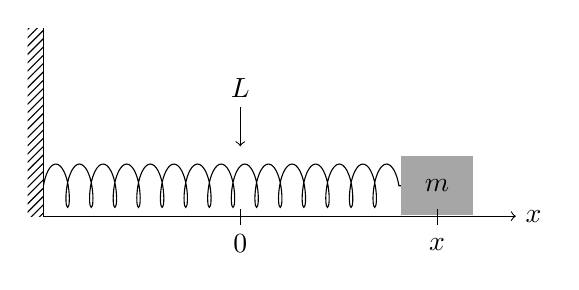
\begin{tikzpicture}
			% Draw Axes
			\draw[->] (0,-.387) -- (6,-.387) node[right] {$x$};
			% Block
			\node[rectangle,fill=gray!70!,inner sep=3mm] (a) at (5,0) {$m$};
			% Spring
			\draw[decoration={aspect=0.3, segment length=3mm, amplitude=2.75mm,coil},decorate] (0,0) -- (a);
			\fill [pattern = north east lines] (-.2,-.387) rectangle (0,2);
			\draw (0,-.387) -- (0,2);
			% Axes Stuff
			\draw (2.5,-0.5) -- (2.5,-0.3) node [below = 2mm] {$0$};
			\draw (5,-0.5) -- (5,-0.3) node[below = 2.5mm] {$x$};
			\draw[->] (2.5,1) -- (2.5,0.5) node[above = 5mm] {$L$};
		\end{tikzpicture}
	\end{center}
	According to Hooke's Law, if the spring is stretched (or compressed) $ x $ units from its natural length, then it exerts a force that is proportional to $x$:
	\[  F = -kx \]
	where $ k $ is a positive constant called the \textit{spring constant}. If we ignore any external resisting forces (due to air resistance or friction) then, by Newton's Second Law we have
	\[ mx''(t) = -kx(t) \qquad \text{or} \qquad mx''(t) + kx(t) = 0 \]
	which is a linear second order differential equation with constant coefficients. Its characteristic equation is $ mr^2 + k = 0 $ with roots $ r = \omega i $, where $ \omega = \sqrt{k/m} $. Thus the general solution is
	\begin{equation}
		x(t) = c_1\cos(\omega t) + c_2\sin(\omega t)
	\end{equation}
	which can also be written as
	\begin{equation}
		x(t) = A\cos(\omega t - \phi)
	\end{equation}
	where $ A $ is the amplitude of the displacement, $ \omega $ is the natural frequency, and $ \phi $ is the phase shift or phase angle of the displacement.\\ \\
	When the displacement is in the form of (2.16) it is usually easier to work with.  However, it's easier to find the constants in (2.15) from the initial conditions than it is to find the amplitude and phase shift in (2.16) from the initial conditions. So, in order to get the equation into the form in (2.16) we will first put the equation in the form in (2.15), find the constants, $ c_1 $ and $ c_2 $ and then convert this into the form in (2.16).\\ \\
	So, assuming that we have $ c_1 $ and $ c_2 $ how do we determine $ A $ and $ \phi $?  Let’s start with (2.16) and use a trig identity to write it as
	\begin{equation}
		x(t) = A\cos(\phi)\cos(\omega t) + A\sin(\phi)\sin(\omega t)
	\end{equation}
	Now, $ A $ and $ \phi $ are constants and so if we compare (2.17) to (2.15) we can see that
	\[ c_1 = A\cos(\phi) \qquad c_2 = A\sin(\phi) \]
	We can find $ A $ in the following way
	\[ c_1^2 + c_2^2 = A^2\cos^2(\phi) + A^2\sin^2(\phi) = A^2 \]
	Taking the square root of both sides and assuming that $ A $ is positive will give
	\[ A = \sqrt{c_1^2 + c_2^2} \]
	Finding $ \phi $ is just as easy. We'll start with
	\[ \frac{c_2}{c_1} = \frac{A\sin(\phi)}{A\cos(\phi)} = \tan(\phi) \]
	Taking the inverse tangent of both sides gives,
	\[ \phi = \tan^{-1}\left( \frac{c_2}{c_1} \right) \]
	Next we'll consider the motion of a spring that is subject to a frictional force or a damping force. An example of a damping force would be a shock absorber on a car. \\ \\
	We assume that the damping force is proportional to the velocity of the mass and acts in the direction opposite to the motion. Thus
	\[ \text{damping force} = -cx'(t) \]
	where $ c $ is a positive constant, called the \textit{damping constant}. So in this case, Newton's Law gives us
	\begin{equation}
		mx''(t) + cx'(t) + kx(t) = 0
	\end{equation}
	Which is another second order linear differential equation with constant coefficients. The characteristic equation is $ mr^2 + cr + k = 0 $. The roots are
	\begin{equation}
		r_{1,2} = \frac{-c \pm \sqrt{c^2 - 4mk}}{2m}
	\end{equation}
	So there will be three different cases for $ r_{1,2} $.\\ \\
	\textbf{Case I} $ c^2 - 4mk > 0 $ (overdamping)\\ \\
	In this case $ r_1 $ and $ r_2 $ are real distinct roots and 
	\[ x(t) = c_1 e^{r_1 t} + c_2 e^{r_2 t} \]
	Since $ c $, $ m $, and $ k $ are all positive, we have $ \sqrt{c^2 - 4mk} < c $, so the roots $ r_1 $ and $ r_2 $ given by (2.19) must both be negative. This shows that $ x \to 0 $ as $ t \to \infty $. Notice that oscillations do not occur.
	
	\begin{center}
		\begin{tikzpicture}
		\draw [thick, red] (0,1.5) .. controls(1,-1.25) and (0,0) .. (5.17,0);
		\draw [<->,thick] (0,2.25) node (yaxis) [left] {$x(t)$}
		|- (5.25,0) node (xaxis) [below] {$t$};
		\node (0,0) [below] {0};
		\end{tikzpicture}
		\captionof{figure}{Overdamping}
	\end{center}

	\noindent \textbf{Case II} $ c^2 - 4mk = 0 $ (critical damping)\\ \\
	In this case $ r_1 $ and $ r_2 $ are equal roots
	\[ r_1 = r_2 = -\frac{c}{2m} \]
	and the solution is given by
	\[ x(t) = (c_1 + c_2 t)e^{-(c/2m)t} \]
	It is similar to Case I, but the damping is just sufficient to suppress vibrations. \\
	
	\noindent \textbf{Case III} $ c^2 - 4mk < 0 $ (underdamping) \\ \\
	In this case the roots are complex
	\[ r_{1,2} = -\frac{c}{2m} \pm i \omega \]
	where
	\[ \omega = \frac{\sqrt{4mk - c^2}}{2m} \]
	The solution is then
	\[ x(t) = e^{-(c/2m)t}(c_1\cos(\omega t) + c_2 \sin(\omega t)) \]
	\begin{center}
		\includegraphics[scale=0.65]{de_1.png}
		
		Figure 2.2: Underdamping
	\end{center}
	We see that there are oscillations that are damped by the factor of $ e^{-(c/2m)t} $. Since $ c > 0 $ and $ m > 0 $, we have $ -(c/2m) < 0 $ so $ e^{-(c/2m)t} \to 0 $ as $ t \to \infty $. This implies that $ x \to 0 $ as $ t \to \infty $; that is, the motion decays to 0 as time increases.
	
	\chapter{Series Solutions to Differential Equations}
	
	In this chapter we will finally be looking at nonconstant coefficient differential equations.  While we won’t cover all possibilities in this chapter we will be looking at two of the more common methods for dealing with this kind of differential equation.
	
	\section{Review: Power Series}
	Before looking at series solutions to a differential equation we will first need to do a cursory review of power series.  A power series is a series in the form,
	\begin{equation}
	f(x) = \sum_{n = 0}^{\infty} a_n (x - x_0)^n
	\end{equation}
	Before proceeding with our review we should probably first recall just what series really are. Recall that series are really just summations. One way to write our power series is then,
	\begin{align*}
	f(x) &= \sum_{n = 0}^{\infty} a_n (x - x_0)^n\\
	&= a_0 + a_1(x-x_0) + a_2(x-x_0)^2 + a_3(x-x_0)^3 + \dots
	\end{align*}
	Notice as well that if we needed to for some reason we could always write the power series as,
	\begin{align*}
	f(x) &= \sum_{n = 0}^{\infty} a_n (x - x_0)^n\\
	&= a_0 + a_1(x-x_0) + a_2(x-x_0)^2 + a_3(x-x_0)^3 + \dots\\
	&= a_0 + \sum_{n = 1}^{\infty} a_n (x - x_0)^n
	\end{align*}
	All that we’re doing here is noticing that if we ignore the first term (corresponding to $ n = 0 $) the remainder is just a series that starts at $ n = 1 $. When we do this we say that we've stripped out the $ n = 0 $, or first, term.\\ \\
	Now, since power series are functions of $ x $ and we know that not every series will in fact exist, it then makes sense to ask if a power series will exist for all $ x $. This question is answered by looking at the convergence of the power series. We say that a power series converges for $ x = c $ if the series,
	\[ \sum_{n = 0}^{\infty} a_n(c - x_0)^n \]
	converges. Recall that this series will converge if the limit of partial sums,
	\[ \lim_{N\to\infty} \sum_{n}^{N} a_n(c-x_0)^n \]
	exists and is finite. In other words, a power series will converge for $ x = c $ if 
	\[ \sum_{n = 0}^{\infty} a_n(c - x_0)^n \]
	is a finite number. With this we now know that power series are guaranteed to exist for at least one value of $ x $. We have the following fact about the convergence of a power series.\\ \\
	\textbf{Fact} Given a power series, (4.1), there will exist a number $ 0 \leq \rho \leq \infty $ so that the power series will converge for $ |x - x_0| < \rho $ and diverge for $ |x - x_0| > \rho $ . This number is called the \textit{radius of convergence}. Determining the radius of convergence for most power series is usually quite simple if we use the ratio test.\\ \\
	\textbf{Ratio Test}\\
	Given a power series, compute 
	\[ L = |x - x_0| \lim_{n\to\infty} \left| \frac{a_{n+1}}{a_n} \right| \]
	then,
	
	\begin{center}
		\begin{tabular}{lll}
			$ L < 1 $ & $ \Rightarrow $ & the series converges\\
			$ L > 1 $ & $ \Rightarrow $ & the series diverges\\
			$ L = 1 $ & $ \Rightarrow $ & the series may converge or diverge
		\end{tabular}
	\end{center}
	
	\noindent \textbf{Example} Determine the radius of convergence for the following power series
	\[ \sum_{n = 0}^{\infty} \frac{(-3)^n}{n 7^{n+1}}(x-5)^n \]
	\textbf{Solution}\\
	In this case we have
	\[ a_n =  \frac{(-3)^n}{n 7^{n+1}} \qquad a_{n+1} = \frac{(-3)^{n+1}}{(n+1)7^{n+2}} \]
	Using the ratio test then gives
	\begin{align*}
	L &= |x-5|\lim_{n\to\infty} \left| \frac{(-3)^{n+1}}{(n+1)7^{n+2}} \frac{n 7^{n+1}}{(-3)^n} \right|\\
	&=|x-5| \lim_{n\to\infty} \left| \frac{-3}{7(n+1)} \frac{n}{1} \right|\\
	&= \frac{3}{7}|x-5|
	\end{align*}
	Thus the radius of convergence is $ \displaystyle{\frac{7}{3}} $.\\ \\
	Next we need to talk about index shifts.  As we will see eventually we are going to want our power series written in terms of $ (x-x_0)^n $ and they often won't, initially at least, be in that form. To get them into the form we need we will need to perform an index shift.\\ \\
	\textbf{Example } Write the following as a series that starts at $ n = 0 $ instead of $ n = 3 $.
	\[ \sum_{n = 3}^{\infty} n^2 a_{n-1}(x+4)^{n+2} \]
	\textbf{Solution}\\
	An index shift is a fairly simple manipulation to perform. First we will notice that if we define $ i=n-3 $ then when $ n = 3 $ we will have $ i = 0 $. So what we'll do is rewrite the series in terms of $ i $ instead of $ n $. We can do this by noting that $ n=i+3 $. So, everywhere we see an $ n $ in the actual series term we will replace it with an $ i + 3 $. Doing this gives,
	\begin{align*}
	\sum_{n = 3}^{\infty} n^2 a_{n-1} (x+4)^{n+2} &= \sum_{i = 0}^{\infty} (i+3)^2 a_{i + 3 - 1} (x+4)^{i + 3 - 2}\\
	&= \sum_{i = 0}^{\infty} (i+3)^2 a_{i+2} (x+4)^{i+5}
	\end{align*}
	The upper limit won't change in this process since infinity minus three is still infinity.\\ \\
	The final step is to realize that the letter we use for the index doesn't matter and so we can just switch back to $ n $'s.
	\[ \sum_{n = 3}^{\infty} n^2 a_{n-1} (x+4)^{n+2} = \sum_{n = 0}^{\infty} (n+3)^2 a_{n+2} (x+4)^{n+5} \]
	Now, we usually don't go through this process to do an index shift. All we do is notice that we dropped the starting point in the series by 3 and everywhere else we saw an $ n $ in the series we increased it by 3. In other words, all the $ n $'s in the series move in the opposite direction that we moved the starting point.
	
	\section{Series Solutions to Differential Equations}
	
	The basic idea to finding a series solution to a differential equation is to assume that we can write the solution as a power series in the form,
	\begin{equation}
	y(x) = \sum_{n=0}^{\infty} a_n (x-x_0)^n
	\end{equation}
	and then try to determine what the $ a_n $'s need to be. We will only be able to do this if the point $ x = x_0 $, is an ordinary point. We will usually say that (4.2) is a series solution around $ x = x_0 $.\\ \\
	Let's start with a simple example\\ \\
	\textbf{Example} Determine a series solution to the differential equation about $ x_0 = 0 $
	\[ y'' + y = 0 \]
	\textbf{Solution}\\
	Lets start by defining $ y(x) $
	\[ y(x) = \sum_{n=0}^{\infty} a_n x^n \]
	We will need to plug this into our differential equation so we'll need to find a couple of derivatives.
	\[ y'(x) = \sum_{n=1}^{\infty} n a_n x^{n-1} \qquad y''(x) = \sum_{n=2}^{\infty} n (n-1) a_n x^{n-2} \]
	So, plug these into our differential equation. Doing this gives, 
	\[ \sum_{n=2}^{\infty} n (n-1) a_n x^{n-2} + \sum_{n=0}^{\infty} a_n x^n = 0 \]
	The next step is to combine everything into a single series. To do this requires that we get both series starting at the same point and that the exponent on the $ x $ be the same in both series. \\ \\
	We will always start this by getting the exponent on the $ x $ to be the same. It is usually best to get the exponent to be an $ n $. The second series already has the proper exponent and the first series will need to be shifted down by 2 in order to get the exponent up to an $ n $.\\ \\
	Shifting the first power series gives us,
	\[ \sum_{n = 0}^{\infty} (n+2)(n+1)a_{n+2} x^n + \sum_{n = 0}^{\infty} a_n x^n = 0 \]
	Nice! Notice that in the process of the shift we also got both series starting at the same place. This won't always happen, but when it does we'll take it. We can now add up the two series. This gives,
	\[ \sum_{n=0}^{\infty} \big[(n+2)(n+1)a_{n+2} + a_n\big]x^n = 0 \]
	Now recalling the fact from the power series review section we know that if we have a power series that is zero for all $ x $ (as this is) then all the coefficients must have been zero to start with. This gives us the following,
	\[ (n+2)(n+1)a_{n+2} + a_n = 0 \]
	This is called the \textit{recurrence relation} and notice that we included the values of $ n $ for which it must be true. We will always want to include the values of $ n $ for which the recurrence relation is true since they won't always start at $ n = 0 $ as it did in this case.\\ \\
	Now let's recall what we were after in the first place. We wanted to find a series solution to the differential equation. In order to do this we needed to determine the values of the $ a_n $'s. We are almost to the point where we can do that. The recurrence relation has two different $ a_n $'s in it so we can't just solve this for $ a_n $ and get a formula that will work for all $ n $. We can however, use this to determine what all but two of the $ a_n $'s are.\\ \\
	To do this we first solve the recurrence relation for the $ a_N $ that has the largest subscript. Doing this gives,
	\[ a_{n+2} = -\frac{a_n}{(n+2)(n+1)} \]
	Now, at this point we just need to start plugging in some value of $ n $ and see what happens,
	\begin{align*}
	n&=0	&  a_2&=\frac{-a_0}{(2)(1)}		&  n&=1		& a_3 &= \frac{-a_1}{(3)(2)}\\
	n&=2	&  a_4&=\frac{-a_2}{(4)(3)}		&  n&=3		& a_5 &= \frac{-a_3}{(5)(4)}\\
	n&=4	&  a_6&=\frac{-a_4}{(6)(5)}		&  n&=5		& a_7 &= \frac{-a_5}{(7)(6)}\\
	&		&	&\qquad \vdots 				&	&		& & \qquad \vdots\\
	&		&	a_{2k} &= \frac{(-1)^k a_0}{(2k)!} 		& & &a_{2k+1} &= \frac{(-1)^k a_1}{(2k+1)!}
	\end{align*}
	Notice that at each step we always plugged back in the previous answer so that when the subscript was even we could always write the $ a_n $ in terms of $ a_0 $ and when the coefficient was odd we could always write the $ a_n $ in terms of $ a_1 $. Also notice that, in this case, we were able to find a general formula for $ a_n $'s with even coefficients and $ a_n $'s with odd coefficients. This won't always be possible to do.\\ \\
	Now that we've got formulas for the $ a_n $'s let's get a solution. The first thing that we'll do is write out the solution with a couple of the $ a_n $'s plugged in.
	\begin{align*}
	y(x) &= \sum_{n = 0}^{\infty} a_x x^n\\
	&= a_0 + a_1x + a_2x^2 + a_3x^3 + \ldots + a_{2k} x^{2k} + a_{2k+1} x^{2k+1} + \ldots\\
	&= a_0 + a_1x  - \frac{a_0}{2!}x^2 - \frac{a_1}{3!}x^3 + \dots + \frac{(-1)^k a_0}{(2k)!} x^{2k} + \frac{(-1)^k a_1}{(2k+1)!} x^{2k+1} + \ldots
	\end{align*}
	The next step is to collect all the terms with the same coefficient in them and then factor out that coefficient.
	\begin{align*}
	y(x) &= a_0 \left( 1 - \frac{x^2}{2!} + \ldots + \frac{(-1)^k x^{2k}}{(2k)!} + \ldots \right) + a_1 \left( x - \frac{x^3}{3!} + \ldots + \frac{(-1)^k}{(2k+1)!} x^{2k+1} + \dots \right)\\
	&= a_0 \sum_{k = 0}^{\infty}  \frac{(-1)^k}{(2k)!} x^{2k} + a_1 \sum_{k=0}^{\infty} \frac{(-1)^k a_1}{(2k+1)!} x^{2k+1}
	\end{align*}
	In the last step we also used the fact that we knew what the general formula was to write both portions as a power series. This is also our solution. Since this was a fairly simple differential equation, we could have solved it using techniques in the previous chapter. But we'll just use it to check our work. If we were to work it out, we get
	\[ y(x) = c_1 \cos(x) + c_2 \sin(x) \]
	Solutions to second order differential equations consist of two separate functions each with an unknown constant in front of them that are found by applying any initial conditions. So, the form of our solution is exactly what we want to get. Also recall that the following Taylor series,
	\[ \cos(x) = \sum_{k = 0}^{\infty}  \frac{(-1)^k}{(2k)!} x^{2k} \qquad \sin(x) = \sum_{k=0}^{\infty} \frac{(-1)^k a_1}{(2k+1)!} x^{2k+1}  \]
	So our solution was correct.
	
	\chapter{Laplace Transforms}
	In this chapter we will be looking at how to use Laplace transforms to solve differential equations. There are many kinds of transforms out there in the world. Laplace transforms and Fourier transforms are probably the main two kinds of transforms that are used. As we will see in later sections we can use Laplace transforms to reduce a differential equation to an algebra problem. The algebra can be messy on occasion, but it will be simpler than actually solving the differential equation directly in many cases. Laplace transforms can also be used to solve initial value problems that we can't use any previous method on.\\ \\
	For ``simple'' differential equations such as those in the first few sections of the last chapter Laplace transforms will be more complicated than we need. In fact, for most homogeneous differential equations such as those in the last chapter Laplace transforms is significantly longer and not so useful. Also, many of the 	``simple'' nonhomogeneous differential equations that we saw in the Undetermined Coefficients and Variation of Parameters are still simpler (or at the least no more difficult than Laplace transforms) to do as we did them there. However, at this point, the amount of work required for Laplace transforms is starting to equal the amount of work we did in those sections. \\ \\
	Laplace transforms comes into its own when the forcing function in the differential equation starts getting more complicated.  In the previous chapter we looked only at nonhomogeneous differential equations in which $ g(t) $ was a fairly simple continuous function. In this chapter we will start looking at $ g(t) $'s that are not continuous. It is these problems where the reasons for using Laplace transforms start to become clear. We will also see that, for some of the more complicated nonhomogeneous differential equations from the last chapter, Laplace transforms are actually easier on those problems as well.
	
	\section{The Definition}
	Before we start with the definition of the Laplace transform we need to get another definition out of the way. A function is called \textit{piecewise continuous} on an interval if the interval can be broken into a finite number of subintervals on which the function is continuous on each open subinterval (i.e. the subinterval without its endpoints) and has a finite limit at the endpoints of each subinterval. In other words, a piecewise continuous function is a function that has a finite number of breaks in it and doesn't blow up to infinity anywhere.
	
	\noindent \textbf{Definition}\\
	 Suppose that $ f(t) $ is a piecewise continuous function. The Laplace transform of $ f(t) $ is denoted $ \L\{f(t)\} $ and defined as
	\begin{equation}
		\L\{f(t)\} = \int\limits_{0}^{\infty} e^{-st}f(t)\,dt
	\end{equation}
	There is an alternate notation for Laplace transforms.  For the sake of convenience we will often denote Laplace transforms as,
	\[ \L\{f(t)\} = F(s) \]
	What the Laplace transform does is takes a function of a real variable $ t $, to a function of a complex variable $ s $.\\ \\
	\noindent \textbf{Example} Compute $ \L\{e^{at}\} $\\ \\
	\noindent \textbf{Solution}\\
	All we need to do is plug our $ f(t) $ into the definition
	\[ \L\{e^{at}\} = \int\limits_{0}^{\infty} e^{-st} e^{at}\,dt = \int\limits_{0}^{\infty} e^{(a-s)t}\,dt \]
	At this point we recall that to solve an improper integral we need to take a limit of our dummy variable as it goes to $ \infty $.
	\begin{align*}
		\int\limits_{0}^{\infty} e^{(a-s)t}\,dt &= \lim_{n\to\infty} \left[ \int\limits_{0}^{n} e^{(a-s)t}\,dt \right]\\
		&= \lim_{n\to\infty} \left[ \frac{1}{a-s} e^{(a-s)t} \Big|_{0}^{n}\right]\\
		&= \lim_{n\to\infty} \left[\left( \frac{1}{a-s}e^{(a-s)(n)} \right) - \left( \frac{1}{a-s}e^{(a-s)(0)} \right) \right]\\
		&= 0 - \frac{1}{a-s} \qquad a -s < 0\\
		&= \frac{1}{s- a} \qquad s > a
	\end{align*}
	
	\noindent These integrals can get pretty messy! Thankfully, someone has already done the dirty work and provided this nifty table of some of the more commonly used transforms.
	
	\begin{center}
	\begin{tabular}{ll}
		$ f(t) $ & $ F(s) = \L\{f(t)\} $ \\ \midrule
		1 & $ \displaystyle{\frac{1}{s}}, \quad s > 0 $\\ \\
		$ e^{at} $ & $ \displaystyle{\frac{1}{s-a}}, \quad s > a $ \\ \\
		$ t^n $ & $ \displaystyle{\frac{n!}{s^{n+1}}}, \quad s> 0 $ \\ \\
		$ \sin(bt) $ & $ \displaystyle{\frac{b}{s^2 + b^2}}, \quad s > 0 $ \\ \\
		$ \cos(bt) $ & $ \displaystyle{\frac{s}{s^2 + b^2}}, \quad s > 0 $ \\ \\
		$ e^{at} t^n $ & $ \displaystyle{\frac{n!}{(s-a)^{n+1}}}, \quad s > a $ \\ \\
		$ e^{at}\sin(bt) $ & $ \displaystyle{\frac{b}{(s-a)^2 + b^2}}, \quad s > a $ \\ \\
		$ e^{at}\cos(bt) $ & $ \displaystyle{\frac{s-a}{(s-a)^2 + b^2}}, \quad s > a $ \\ \\
	\end{tabular}
	\end{center}
	And here are some properties of the Laplace Transform
	\begin{align*}
		& \L\{f(t) + g(t)\} = \L\{f(t)\} + \L\{g(t)\}\\
		& \L\{cf(t)\} = c\L\{f(t)\} \quad \text{ for any constant } c\\
		& \L\{e^{at} f(t)\} = F(s-a)\\
		& \L\{f'(t)\} = sF(s) - f(0)\\
		& \L\{f''(t)\} = s^2F(s) - sf(0) - f'(0)\\
		& \L\{f^{(n)}(t)\} = s^n F(s) - s^{n-1}f(0) - s^{n-2}f'(0) - \ldots - f^{(n-1)}(0)\\
		& \L\{t^nf(t)\} = (-1)^n \frac{d^n}{ds^n} (F(s))
	\end{align*}
	 
	\section{Inverse Laplace Transforms}
	Finding the Laplace transform of a function is not terribly difficult if we've got a table of transforms in front of us to use as we saw in the last section. What we would like to do now is go the other way. We are going to be given a transform, $ F(s) $, and ask what function (or functions) did we have originally. This can be a more complicated and lengthy process than taking transforms. In these cases we say that we are finding the Inverse Laplace Transform of $ F(s) $ and use the following notation
	\[ f(t) = \L^{-1}\{F(s)\} \]
	
	
	\noindent \textbf{Example} Find the inverse transform of
	\[ F(s) = \frac{6}{s} - \frac{1}{s+8} + \frac{4}{s-3} \]
	\textbf{Solution}\\
	From the denominator of the first term it looks like the first term is just a constant. The correct numerator for this term is a ``1'' so we'll just factor the 6 out before taking the inverse transform. The second term appears to be an exponential with $ a = 8 $ and the numerator is exactly what it needs to be. The third term also appears to be an exponential, only this time $ a = 3 $ and we'll need to factor the 4 out before taking the inverse transforms.\\ \\ 
	So, with a little more detail than we'll usually put into these,
	\begin{align*}
	F(s) &= 6\frac{1}{s} - \frac{1}{s - 8}+ 4\frac{1}{s - 3}\\
		f(t) &= 6 (1) - e^{8t} + 4(e^{3t})\\
		&= 6 - e^{8t} + 4e^{3t}
	\end{align*}
	So, probably the best way to identify the transform is by looking at the denominator. If there is more than one possibility use the numerator to identify the correct one.  Fix up the numerator if needed to get it into the form needed for the inverse transform process. Finally, take the inverse transform.
	
	\section{Solving Initial Value Problems with Laplace Transforms}
	
	Finally, we now get to use our new skills from the last two sections and actually apply these transforms to solve differential equations! Hurray! Let's start with an example\\ \\
	\textbf{Example} Solve the initial value problem using Laplace transforms
	\[ y'' - 10y' + 9y = 5t \qquad y(0) = -1  \quad y'(0) = 2\]
	\textbf{Solution}\\
	The first step is to take a transform of both sides, using the properties of the Laplace transform
	\[ \L\{y''\} - 10\L\{y'\} + 9\L\{y\} = 5\L\{t\} \]
	Using the appropriate formulas from our table of Laplace transforms gives us the following.
	\[ s^2 Y(s) - sy(0) - y'(0) - 10(sY(s) - y(0)) + 9Y(s) = \frac{5}{s^2} \]
	Plug in the initial conditions and collect all the terms that have a $ Y(s) $ in them.
	\[ Y(s)(s^2 - 10s + 9) + s -12 = \frac{5}{s^2} \]
	Then solve for $ Y(s) $,
	\[ Y(s) = \frac{5}{(s^2)(s-9)(s-1)} + \frac{12 - s}{(s-9)(s-1)} = \frac{5 + 12s^2 - s^3}{s^2(s-9)(s-1)} \]
	At this point it's convenient to recall just what we're trying to do. We are trying to find the solution, $ y(t) $, to an IVP. What we've managed to find at this point is not the solution, but its Laplace transform. So, in order to find the solution all that we need to do is to take the inverse transform.\\ \\
	We need to split this fraction up into smaller ones and take inverse Laplaces of those, so we need to do partial fraction decomposition
	\[ Y(s) = \frac{5 + 12s^2 - s^3}{s^2(s-9)(s-1)} = \frac{A}{s} + \frac{B}{s^2} + \frac{C}{s-9} + \frac{D}{s-1} \]
	Setting numerators equal gives,
	\[ 5 + 12s^2 - s^3 = As(s-9)(s-1) + B(s-9)(s-1) + Cs^2(s-1) + Ds^2(s-9) \]
	Picking appropriate values of s and solving for the constants gives,
	\begin{center}
		\begin{tabular}{lcll}
			$ s = 0 $ & $ 5 = 9B $  & $ \Rightarrow $ & $ \displaystyle{B = \frac{5}{9}} $ \\ \\
			$ s = 1 $ & $ 16 = -8D $ & $ \Rightarrow $ & $ \displaystyle{D = -2} $  \\ \\
			$ s = 9 $   & $ 248 = 648C $ & $ \Rightarrow $ & $ \displaystyle{C = \frac{31}{81}}$ \\ \\
			$ s = 2 $ & $ 45 = -14A + \displaystyle{\frac{4345}{81}} $ & $ \Rightarrow $ & $ \displaystyle{A =\, \frac{50}{81}} $
		\end{tabular}
	\end{center}
	Plugging in the constants gives,
	\[ Y(s) = \frac{50/81}{s} + \frac{5/9}{s^2} + \frac{31/81}{s - 9} - \frac{2}{s - 1} \]
	Finally taking the inverse transform gives us the solution to the initial value problem
	\[ y(t) = \frac{50}{81} + \frac{5}{9}t + \frac{31}{81}e^{9t} - 2e^t \]
	That was a fair amount of work for a problem that probably could have been solved much quicker using the techniques from the previous chapter. The point of this problem however, was to show how we would use Laplace transforms to solve an IVP.\\ \\
	There are a couple of things to note here about using Laplace transforms to solve an IVP.  First, using Laplace transforms reduces a differential equation down to an algebra problem.  In the case of the last example the algebra was probably more complicated than the straight forward approach from the last chapter.  However, in later problems this will be reversed.  The algebra, while still very messy, will often be easier than a straight forward approach.\\ \\
	Second, unlike the approach in the last chapter, we did not need to first find a general solution, differentiate this, plug in the initial conditions and then solve for the constants to get the solution.  With Laplace transforms, the initial conditions are applied during the first step and at the end we get the actual solution instead of a general solution.
	
	




	

	\addcontentsline{toc}{chapter}{}
	\pagestyle{plain}

\end{document}
